\documentclass[transmag]{IEEEtran}
\usepackage{latexsym}
\usepackage{graphicx}
\usepackage{amsfonts,amssymb,amsmath}
\usepackage{hyperref}
\graphicspath{ {./images/} }
\renewcommand\IEEEkeywordsname{Keywords}
\usepackage{pdfpages}
\def\BibTeX{{\rm B\kern-.05em{\sc i\kern-.025em b}\kern-.08em T\kern-.1667em\lower.7ex\hbox{E}\kern-.125emX}}
\usepackage{float}
\usepackage{aliascnt}
\newaliascnt{eqfloat}{equation}
\newfloat{eqfloat}{h}{eqflts}
\floatname{eqfloat}{Equation}
\usepackage{cancel}

\begin{document}

\title{\textsc{Robot Manipulator Design Assignment}}

\clearpage\thispagestyle{empty}

\author{Souto T.L.

\\
\\
\\

\begin{centering}
\vspace{20mm}

\includegraphics[scale=0.25]{massey-png}
\end{centering}



\thanks{This paper is a Individual design Project and It is part of the second assignment of the course Master of engineering - Mechatronics at Massey university, Auckland.

An electronic version of this report can be found by following this \textcolor{blue}{\href{https://thiagosoutogit.github.io/Masters/Pages/Automation/Assessment02RoboticArm.html}{link}}, and the programming documentation can be found by following this \textcolor{blue}{\href{https://thiagosoutogit.github.io/Robot-Manipulator/}{link}}, also a GitHub repository with all the files used in this project is available \textcolor{blue}{\href{https://github.com/ThiagoSoutoGit/Robotic-Manipulator-Files}{here}}. 

Thiago Lima Souto is a student register under the number 19044686 at Massey university. Questions, comments or communications can be addressed via email \color{blue}\href{mailto:thiago.souto@yahoo.com.br}{thiago.souto@yahoo.com.br}

\textcolor{red}{Please Check the links.}
}}


\IEEEtitleabstractindextext{\begin{abstract}
In this paper is reported the design of a robotic manipulator with four degrees of freedom on a fixed platform placed on a flat surface, It's able to be integrated with a robotic gripper also designed. The objective of this robotic system is to pick an object from a shelf or from the wall and place it onto a horizontal surface.
Several tools were used to accomplish the objective of this project. For the calculations of forward and inverse kinematics Python programming language and the Pycharm IDE(Integrated Development Environment) were used, for modelling the robotic system SolidWorks, to simulate OpenModelica was chosen. The description of the design and how this tools were applied as well as why they were chosen is explained here.
As part of this report, a documentation website and a electronic report were built as well as a GitHub repository with all the files.

\end{abstract}



\begin{IEEEkeywords}
robotic systems, forward kinematics, inverse kinematics 
\end{IEEEkeywords}
}

\maketitle
\thispagestyle{empty}

\clearpage
\newpage

\clearpage\thispagestyle{empty}
\onecolumn
\tableofcontents

\clearpage
\newpage

\twocolumn








\section{INTRODUCTION}

Industrial robot systems as well as computer-aided design and manufacturing (CAD and CAM) are leading the industrial automation. \cite{ref1}

The mechanical manipulator is the most important form of the industrial robot and the localization of objects in the three-dimensional space is one of the most important aspect of the mechanical manipulator. Links, parts, tools, other objects on the manipulator environment and the motion of these objects are the subjects of study of Kinematics,  as well as all the geometrical and time-based properties of the motion, with no regards to the forces applied that causes it.

The two basic problems in the study of mechanical manipulation are forward and inverse kinematics, the first computes the position and orientation of the end-effector on the manipulator and the second calculates all possible sets of joint angles that could be used  a given position and orientation. 

Nowadays, CAD and CAM advanced software's are of easy access and used to design, simulate and calculate all that is necessary for modern robot design.

The main objective of this assessment is to design a robotic manipulator with a fixed platform and flat surface, that is able to be integrated with a robot gripper for picking an object vertical wall/shelf and placing it onto a horizontal surface. 

To accomplish this objective a robot system is proposed after this introduction followed by the manipulator and other components design. The forward and inverse kinematics of the robot system are studied with manual calculations as well as computed calculations. A Model with correct dimensions and a simulation of the proposed robot are made using Solidworks and OpenModelica. Finally, the results are discussed and the report is concluded.






 

\section{Robot System Initial Proposal}

Aiming on the objective of designing a robot system, basically, capable of picking an object from a shelf and placing it onto a horizontal surface, the system proposed is a 4$dof$ (degrees of freedom, calculated using Grubler's formula) robot manipulator, consisting of a fixed base, a rotating base, two solid links and a toll, as shown in the Figure \ref{Model}.

\begin{eqfloat}
\begin{equation}
\begin{matrix}
dof = m(N-1-J) + \sum_{i=1}^{J} f_i \\
dof = 6(5-1-4) + 4 \\
dof = 4 
\end{matrix}
\end{equation}
\begin{center}
Gluber's Formula
\end{center}
Where,

$N$ = number of bodies, counting ground as one body.

$J$ = Number of joints.

$m$ = 6 for spatial bodies.

$f_i$ = degrees of freedom of each joint.
\end{eqfloat}


To control the joints four brushless AC motors are used. The motors have attached a magnetic absolute encoder and a integrated controller.
At the end of the system there is a simple gripper making the robotic manipulator able to pickup an place the object.  



\begin{figure}
\centerline{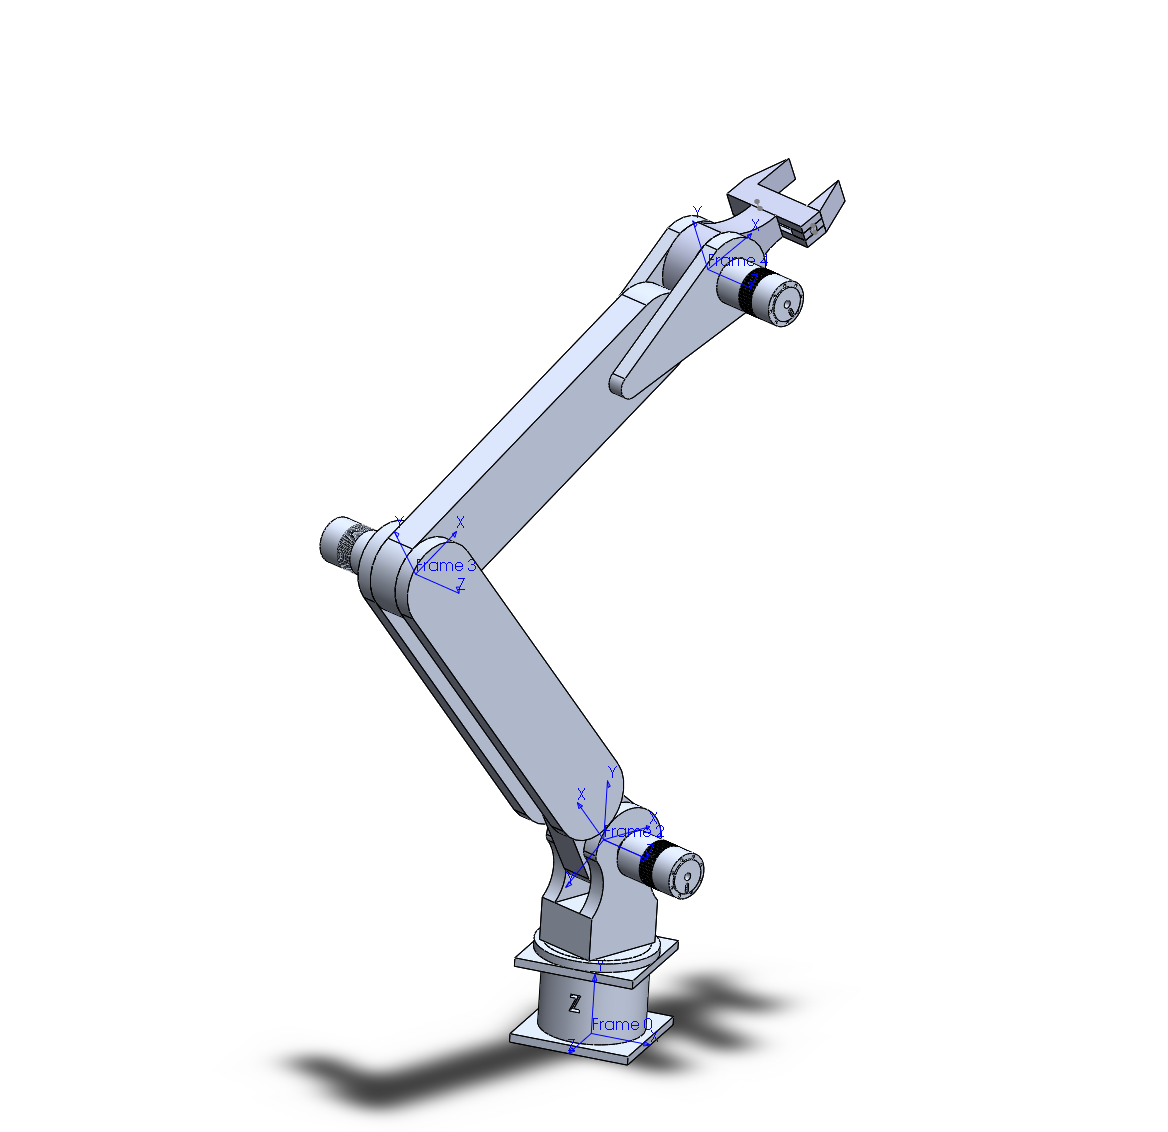
\includegraphics[width=3.5in]{./images/Model}}
\caption{Proposed robot manipulator system.\label{Model}}
\end{figure}



\section{Manipulator Design}


\subsection{Robot Arms}
Link 1 and Link 2 constitute the "arms" of the manipulator, they are designed to maximize the joint angle reach for more flexibility. Also in the rotation base there are two cuts two maximize even further the arms reach as can be seen on Figure \ref{Arms}. In this picture, with the Wireframe view with hidden lines visible, the fourth motor located inside the base can be seen, It is hidden on Figure \ref{Link1Model}.


\begin{figure}
\centerline{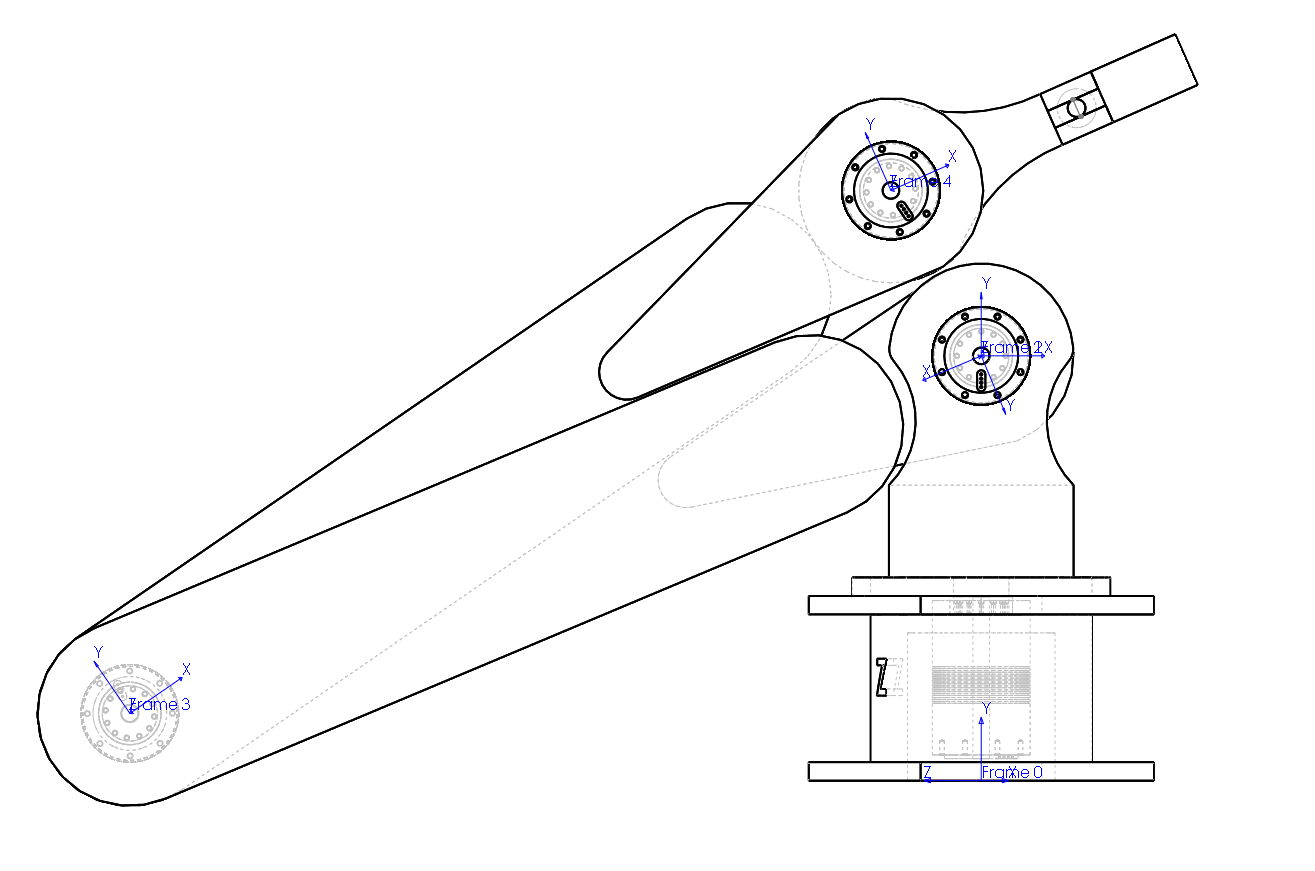
\includegraphics[width=3.5in]{./images/Arms}}
\caption{Arms flexibility on Wireframe view.\label{Arms}}
\end{figure}

\subsection{Robot Gripper}
A gripper capable to hold a 80 mm square object is connected to frame $\{W\}$.
In one of the gripper's claws there is a micro-motor to enable the gripper to hold.
One of the claws of the gripper is attached to a threaded cylinder and then attached to a micro-motor, which will rotate the threaded cylinder and make the claw move. Figure \ref{Gripper} shows the details of the gripper.

\begin{figure}
\centerline{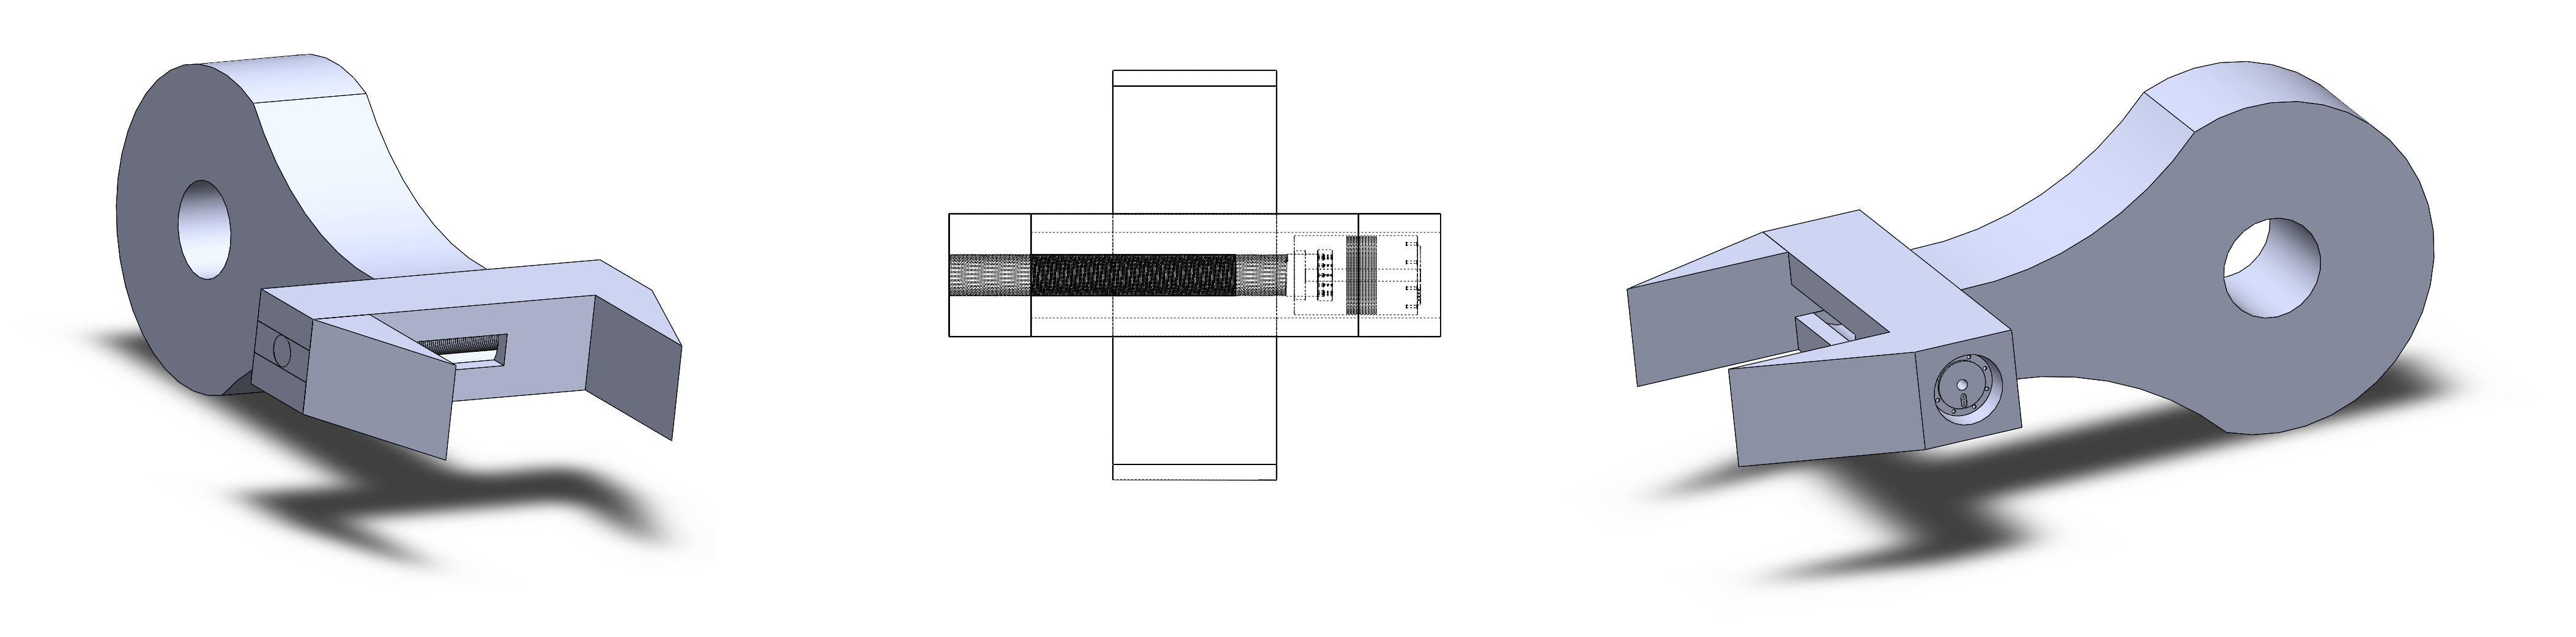
\includegraphics[width=3.5in]{./images/Gripper}}
\caption{Gripper details.\label{Gripper}}
\end{figure}
 

\subsection{Entire Model}

Together with the Arms and the Gripper there is a fixed base and a rotational base. The Soliworks model shown on Figure \ref{Model} the electronics are discussed on the next topic.




\section{Other Components}
The actuator chosen for the project is a complete system with sensors, controller and a motor. It can be used on several applications such as robots and drones, model aircrafts, conveyor belts, sorting and assembly lines, and packing equipment to name some.


\subsection{Motors}

There are various types of motors and key factors need to be taken into account when selecting one for a particular application \cite{ref3}, in this case to control the joints of a robotic manipulator. The main factors are:

\subsubsection{Inertia matching}

The robotic system have to be capable to achieve a required torque to give a load a moment of particular inertia and to achieve a desired angular acceleration. The moment of inertia was calculated using the Iterative Newton-Euler Dynamics Algorithm \cite{ref7}, and this is solved in two parts, first the links velocities and accelerations are iteratively computed across the links applying the Newton-Euler equations to each link, then the forces and torques of interaction and joint actuator torques are computed recursively from the last link to the first.

This calculation was made by simulating the system using a simulation software, OpenModelica. The values for $\tau$ of each joint during the time of the simulation, $15 s$, are shown on Figure \ref{TauJoints}, and, as can be noted, the maximum torque required was $97.9063 N.m$. The simulation was made with the load attached to the system.

\begin{figure}
\centerline{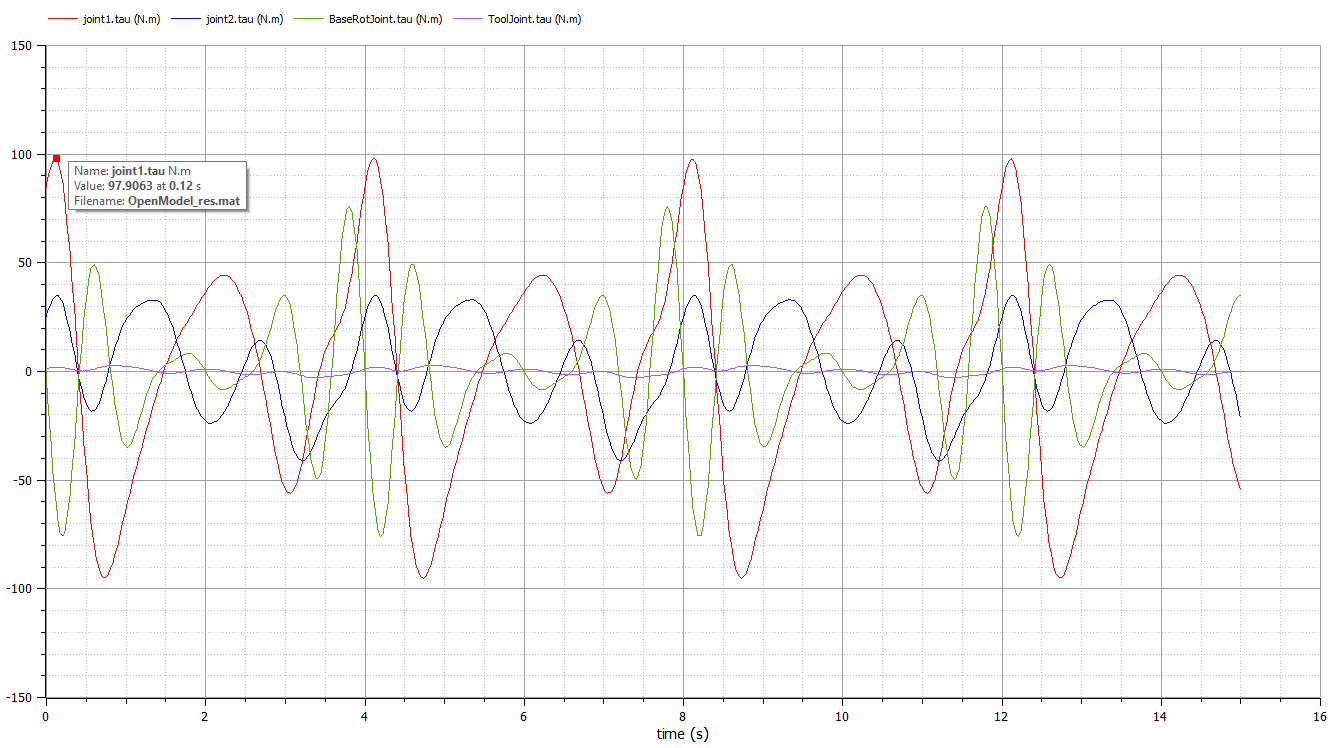
\includegraphics[width=3.5in]{./images/TausJoints}}
\caption{Torque plot for various angles of the 4 joints, Max. 90.7566 N.m.\label{TauJoints}}
\end{figure}

\subsubsection{Torque requirements}

High torque means a mechanism is able to handle heavier loads. The motor used for the modelling is capable of $157 N.m$ and should be able to handle the $97.9063 N.m$ with a $59.0937 N.m$ margin.

\subsubsection{Power requirements}

As well as the torque requirements this project don't require that the motors run at maximum velocity, therefore overheating will not be a problem, and this is one of the main aspects of power requirements for a motor. The total power required is the sum of the power needed to overcome friction and that needed to accelerate the load \cite{ref4}.


After analysing and taking into consideration the aspects discussed above the RDrive 85 motor with rated torque of $108 N.m$ and peak torque of $157 N.m$ and $450W$ of Power was chosen to the task. \cite{ref8} For the gripper a 20 mm diameter motor was used.


 

\begin{figure}
\centerline{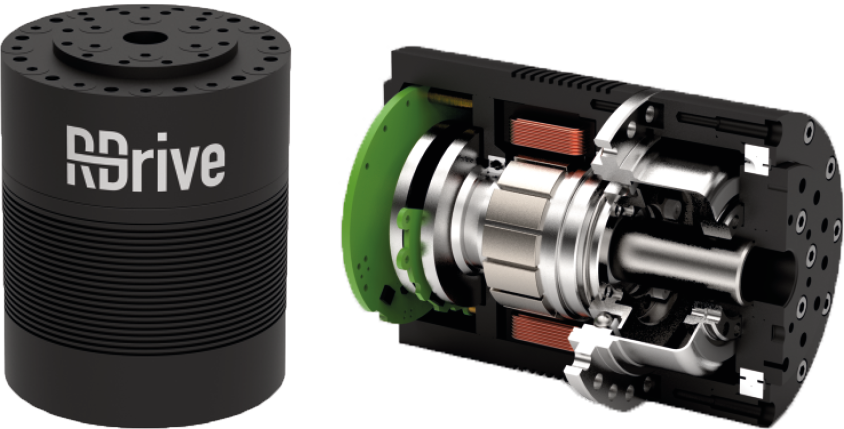
\includegraphics[width=3.5in]{./images/Motor}}
\caption{RDrive motor.\label{Motor}}
\end{figure}



\subsection{Sensors}

To know the angular position of the joints absolute encoders shall be the choice because they give the actual angular position, a unique identification of an angle. The incremental encoders would detect the changes but in relation to some Datum. \cite{ref3}

So with the absolute encoders we can track $\theta_1,\theta_2$, $\theta_3$ and $\theta_4$ and rearrange the links accordingly with the joints angles.

Each motor comes with a 19-bit absolute encoder built-in.


\subsection{Controllers}
Rozum robotics RDrive have an integrated controller supporting CANopen communication encoders.
This motors come with a Python/java API and can be programmed from a control unit like an arduino, a PIC or a STM32 ARM microcontrollers. 
























\section{Forward Kinematic}


To calculate the forward kinematics equation, a Python Class called "FowardKinematics" was created, this Class has two main methods involved on the calculations, the rotation and the translation for the $\hat Z$ and $\hat X$ axis. The parameters for these methods are extracted from the Denavit–Hartenberg parameters at $(1)$, the coordinate systems and also the basic frames $\{B\}$, $\{W\}$ and $\{T\}$, Base, Wrist and Tools respectively are identified on the Figure \ref{Axis}. The size of the links are $l_1 = 230$, $l_2 = 500$, $l_3 = 500$, $l_4 = 180$.

The forward kinematics calculations were confirmed by a python programming code that can be found in the Appendix \ref{appendix-A}. 

\begin{figure}
\centerline{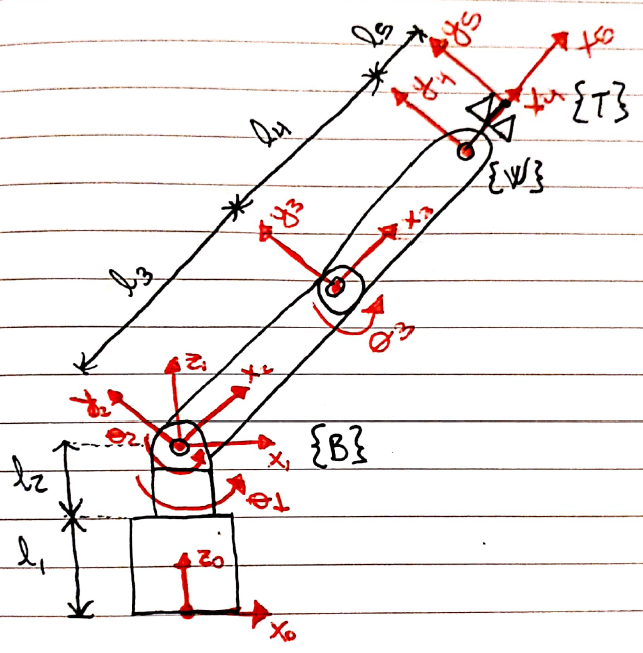
\includegraphics[width=3.5in]{./images/Axis}}
\caption{$\hat Z, \hat Y, \hat X axis, \theta_1, \theta_2, \theta_3, l1, l2, l3$ and $l4$.\label{Axis}}
\end{figure}

The rotation method receives an argument $self$ and $\theta_i$ for the rotation on the $\hat Z$ axis and $\alpha_{i-1}$ for $\hat X$. The $self$ argument is what makes this a method and not just a plain function, this is filled in automatically, when we call this method on the object. So we'll just provide one argument, and the fact that it's being called on the method will provide the first argument, self. It will then build a $sympy$ symbolic matrix and passes the $self$ argument to the method to be put in place, if no arguments are passed default values will be put in place as specified in the key word arguments ($\**$ $kwargs$) on the $\_\_init\_\_$ function. A Matrix is then returned after calling the $.evalf()$ function to evaluate.

Like in the rotation method the translation method receives a argument $d_i$ and $a_{i-1}$ to return a matrix that translates in $\hat Z$ and $\hat X$ axis respectively. This class is also detailed in the Appendix \ref{appendix-A}.  

The objective of the forward kinematics is to provide a kinematics equation relating the end-effector orientation and position. This is done by finding the Denavit–Hartenberg parameters and the homogeneous transforms for each step from 0 to 5. These matrix are shown from (2) to (09). Finally, the forward kinematics equation is presented on Equation \ref{Forward Kinematics}.




\begin{eqfloat}
\begin{equation}
\begin{tabular}{c|c|c|c|c}
$i$  & $\alpha_{i-1}$ & $a_{i-1}$ & $d_i$        & $\theta_i$ \\
\hline
1    &  0             &  0         &  $l_1$ & $\theta_1$ \\
2    &  $90^{\circ}$        &  0         &  0     & $\theta_2$ \\
3    &  0             &  $l_2$     &  0     & $\theta_3$ \\
4    &  0             &  $l_3$     &  0     & $\theta_4$ \\
5    &  0             &  $l_4$     &  0     & 0 \\
\end{tabular}
\end{equation}

\begin{center}
Denavit–Hartenberg parameters
\end{center}




\begin{equation}
^0_1T =
\begin{bmatrix}
cos\theta_1 & -sin\theta_1 & 0 & 0   \\
sin\theta_1 & cos\theta_1  & 0 & 0   \\
0           & 0            & 1 & l_1 \\
0           & 0            & 0 & 1   \\
\end{bmatrix}
\end{equation}


\begin{equation}
^1_2T =
\begin{bmatrix}
cos\theta_2 & -sin\theta_2 & 0      & 0   \\
0           & 0            & -1     & 0   \\
sin\theta_2 & cos\theta_2  & 0      & 0   \\
0           & 0            & 0      & 1   \\
\end{bmatrix}
\end{equation}




\begin{equation}
^2_3T =
\begin{bmatrix}
cos\theta_3 & -sin\theta_3 & 0      & l_2 \\
sin\theta_3 & cos\theta_3  & 0      & 0   \\
0           & 0            & 1      & 0   \\
0           & 0            & 0      & 1   \\
\end{bmatrix}
\end{equation}



\begin{equation}
^3_4T =
\begin{bmatrix}
cos\theta_4 & -sin\theta_4 & 0      & l_3 \\
sin\theta_4 & cos\theta_4  & 0      & 0   \\
0           & 0            & 1      & 0   \\
0           & 0            & 0      & 1   \\
\end{bmatrix}
\end{equation}



\begin{equation}
^4_5T =
\begin{bmatrix}
1 & 0 & 0 & l_4  \\
0 & 1 & 0 & 0   \\
0 & 0 & 1 & 0   \\
0 & 0 & 0 & 1   \\
\end{bmatrix}
\end{equation}

\begin{equation}
^0_5T = ^0_1T  ^1_2T  ^2_3T  ^3_4T  ^4_5T => ^0 \cancel{_1T  ^1_2T  ^2_3T  ^3_4T  ^4} _5T = ^0_5T
\label{1-5}
\end{equation}




\begin{equation}
^0_5T =
\begin{bmatrix}
C_1C_{234}
& 
-S_{234}C_1
& 
S_1
& 
C_1(l_2 C_2 + l_3 C_{23} + l_4 C_{234}) \\
&&&&
\\
S_1 C_{234}     
& 
-S_1 S_{234} 
& 
-C_1
& 
 S_1 (l_2 C_2 + l_3 C_{23} + l_4 C_{234})
\\
&&&&
\\
S_{234}
&
C_{234}
&
0
&
l_1 + l_2 S_2 + l_3 S_{23} + l_4 S_{234} 
\\
&&&&
\\
0           & 0            & 0      & 1   \\
\end{bmatrix}
\label{Forward Kinematics}
\end{equation}

\end{eqfloat}










\section{Inverse Kinematics}

There are many methods to find the equations for the inverse kinematic here two methodologies are presented. First let's look at the trigonometric solution. For the trigonometric solution we can draw 2 triangles, on from frame $\{1\}$ to $\{4\}$ and the second one from frame $\{3\}$ to frame $\{5\}$. This way we can study the relation between the angles. 

If we assume $theta_1 = 0$ we can calculate the angle relation between the triangles on Figure \ref{Inverse_triangles} as if they were on the same plane.

\begin{figure}[h]
\centerline{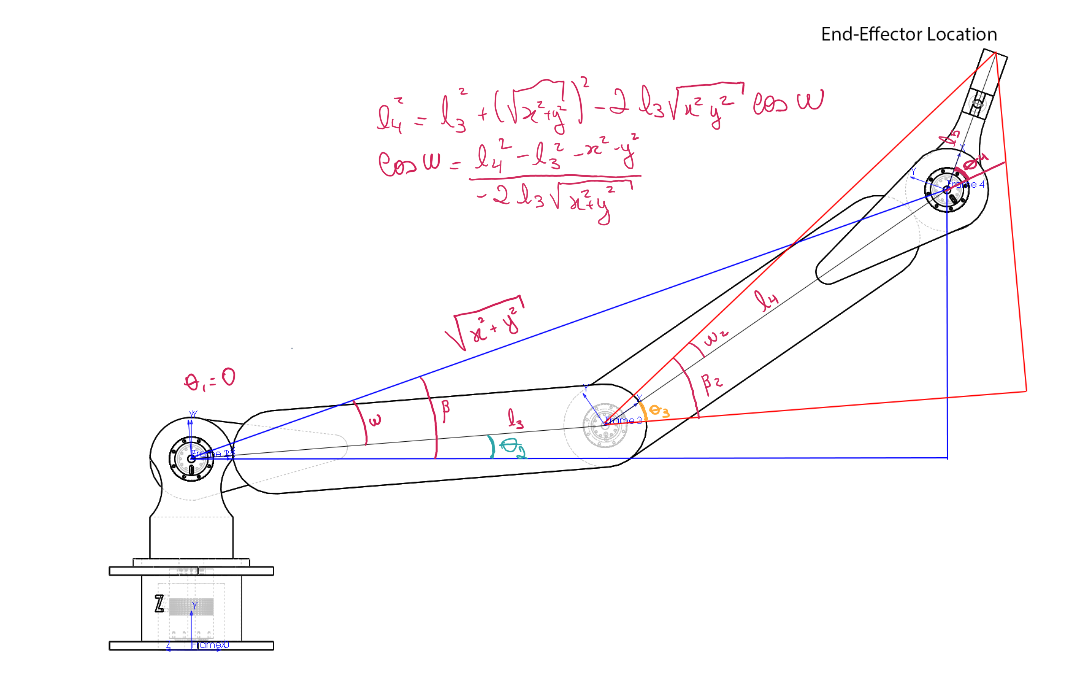
\includegraphics[width=3.5in]{./images/Inverse_triang}}
\caption{Triangles from frame $\{1\}$ to $\{4\}$ and $\{3\}$ to $\{5\}$.\label{Inverse_triangles}}
\end{figure}

To find the hypotenuses of the triangles we have to find $^1_4T$, $^3_5T$ and $^1_5T$. This can be achieved by multiplying both sides of Equation \ref{1-5} by the dependent transpose inverse $T^{-1}$, as shown below.

If we consider Equation \ref{1-5_2}:

\begin{equation}
^0_5T = ^0_1T  ^1_2T  ^2_3T  ^3_4T  ^4_5T
\label{1-5_2}
\end{equation}

and we multiply both sides by $^0_1T^{-1}$ we have,

\begin{equation}
^0_5T {^0_1T}^{-1} = {^0_1T}^{-1} {^0_1T} ^1_2T  ^2_3T  ^3_4T  ^4_5T
\end{equation}

Which is the same as,

\begin{equation}
^1_5T = ^1_2T  ^2_3T  ^3_4T  ^4_5T
\end{equation}

To find $^1_4T$ we can "go" to $^1_5T$ and "coming back" one step by computing the inverse $^4_5T^{-1}$. Then we have,

\begin{equation}
^1_4T = ^1_5T ^4_5T^{-1}
\end{equation}

And for $^3_5T$ from the red triangle we can multiply $^1_2T^{-1}$ and $^2_3T^{-1}$ by $^1_5T$. Then we have,

\begin{equation}
^3_5T = ^1_5T {^1_2T}^{-1}  {^2_3T}^{-1}
\end{equation}


Computing $^1_4T$, calculation made on Appendix \ref{appendix-A},

\begin{equation}
^1_4T = 
\begin{bmatrix}
C_{234} & -S_{234} & 0 & l_2 C_2 + l_3 C_{23} \\
0 & 0 & -1 & 0 \\
S_{234} & C_{234} & 0 & l_2 S_2 + l_3 S_{23} \\
0 & 0 & -1 & 1 \\
\end{bmatrix}
\end{equation}

And $^3_5T$,

\begin{equation}
\begin{matrix}
^3_5T = \\
\\
\begin{bmatrix}
C_{3}C_{34} & S_{3}C_{34} & -S_{34}  & l_2 C_2 - l_2 C_3 C_{34} + L_3 C_{23} + L_4 C_{234} \\
-S_3        & C_3         & 0        & l_2 S_3 \\
S_{34} C_3  & S_3 S_{34}  & cos_{34} & l_2 S_2 - l_2 C_3 S_{34} + L_3 S_{23} + L_4 S_{234}\\
0           & 0           & -1       & 1 \\
\end{bmatrix}
\end{matrix}
\end{equation}






By using the law of cosines which states that, on a triangle $A, B, C$, we have,

\begin{figure}[h]
\centerline{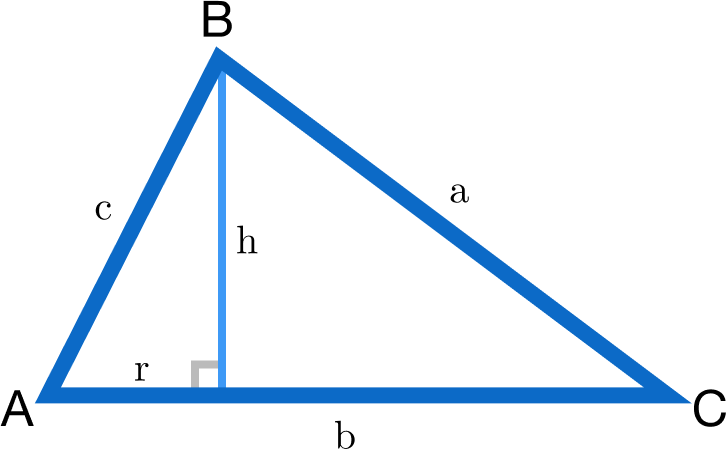
\includegraphics[width=2in]{./images/cosines}}
\caption{Law of cosines.\label{cosines}}
\end{figure}

\begin{equation}
\begin{matrix}
c^2 = \vec{c} . \vec{c} = \\
(\vec{b} - \vec{a}).(\vec{b} - \vec{a}) = \\
b^2 + a^2 - 2\vec{a} . \vec{b} = \\
b^2 + a^2 - 2 ab cosC.
\end{matrix}
\end{equation}

Applying to the blue triangle on Figure \ref{Inverse_triangles},

\begin{equation}
\begin{matrix}
cos\omega = \frac{l_4^2 - l_3^2 - x^2 - y^2}{-2l_3 \sqrt{x^2 + y^2}} \\
\\
sin \omega = \sqrt{1 - {cos \omega}^2}
\end{matrix}
\end{equation}

Therefore,

\begin{equation}
\begin{matrix}
\omega = Atan2(sin\omega, cos\omega) \\
\theta_2 = \beta - \omega
\end{matrix}
\end{equation}

Solving for the red triangle and considering $(x, y)$ as from $^3_5T$, we have, a direct relation to $\theta_3$ by using the relation with the angle $a$ where,

\begin{equation}
\begin{matrix}
a = 180 - \theta_3 \\
cos(a) = cos(180 - \theta_3) = \\
-cos\theta_3\\
\end{matrix}
\end{equation}

then we can have,

\begin{equation}
\begin{matrix}
(\sqrt{x^2 + y^2})^2 = {l_3}^2 +  {l_4}^2 + 2l_3l_4 cos\theta_3 \\
\\
cos\theta_3 = \frac{x^2 + z^2 - {l_3}^2 - {l_4}^2}{2l_3l_4} \\
\\
sin \theta_3 = \sqrt{1 - cos(\omega_2)^2} \\
\\
\theta_3 = Atan2(sin\omega_2, cos\omega_2)
\end{matrix}
\end{equation}


For $\theta_4$ we cannot use the cosine law, instead we have to consider the yellow triangle with $l_5$ as hypotenuses and $x - l_4$ and we have,





\begin{equation}
\begin{matrix}
cos\theta_4 = \frac{x-l_4}{l_5} \\
\\
sin\theta_4 = \sqrt{1 - {cos\theta_4}^2} \\
\\
\theta_4 = Atan2(sin\theta_4, cos\theta_4)
\end{matrix}
\end{equation}


As a proof of the equations for the inverse kinematics a program in python was written using the a simple case where $\theta_2 = 0$, $\theta_3 = 45$ and $\theta_4 = 45$. The results were consistent and the program is exposed on Appendix \ref{appendix-A}.





\section{System Simulation}

OpenModelica is currently the most complete open-source Modelica and FMI based modelling, simulation, optimization, and model-based development environment. Its long-term development is supported by a non-profit organization – the Open Source Modelica Consortium (OSMC). \cite{ref2}

This system was chosen, mainly, because of the open-source aspect, since Mathworks Simulink requires a paid plugin to connect the Solidworks model. Also due to the fact that Its a complete system for simulation modelling, versatile and capable of very complex tasks, much more complex than the current project.

For the modelling simulation parameters, information from the CAD simulator (SolidWorks) regarding to mass, center of mass and moments of inertia, were confronted with the Python simulation and was consistent as shown on Figure \ref{MassProperties} and at the Python programming documentation that can be found on Appendix \ref{appendix-A}. More information about the model is also provided but not included necessary to the link properties at OpenModelica, like density, volume, surface area, among others. The parameters necessary for the model were the length, mass and center of mass, as well as the inertia tensors, as shown on Figure \ref{Link1Parameters}. 



\begin{figure}
\centerline{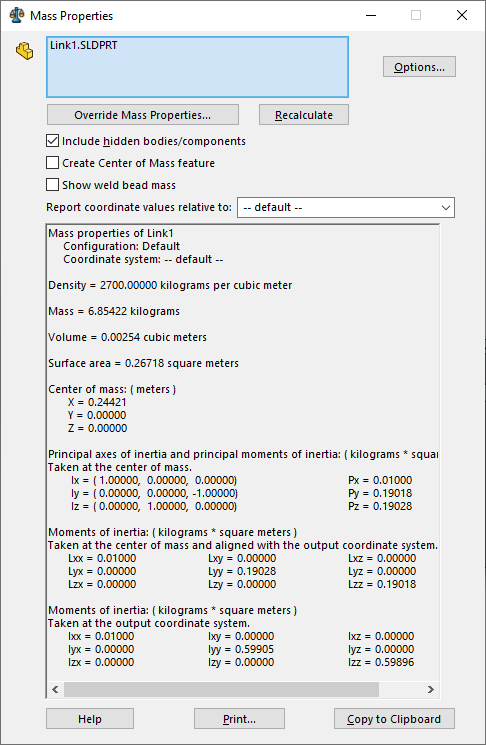
\includegraphics[width=3.5in]{./images/MassProperties}}
\caption{Mass, center of mass and moments of inertia used on the simulation from link1 - SolidWorks.\label{MassProperties}}
\end{figure}


\begin{figure}
\centerline{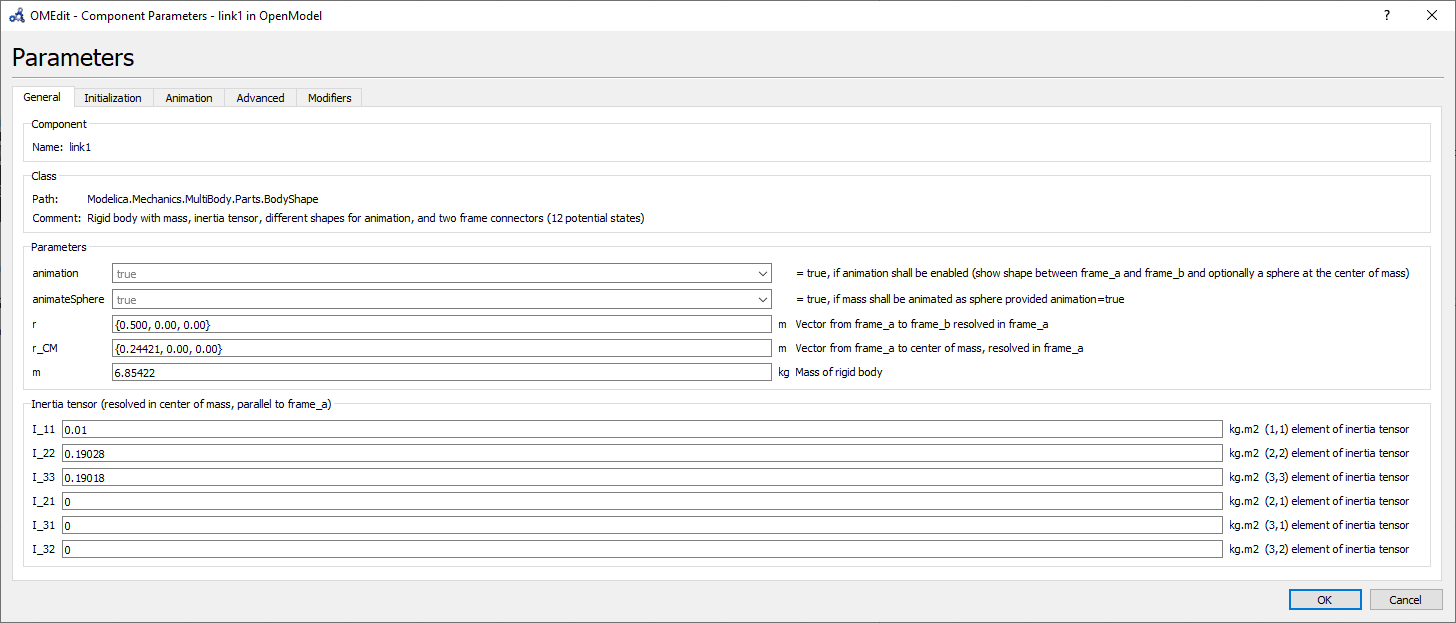
\includegraphics[width=3.5in]{./images/Link1Parameters}}
\caption{OpenModelica, link1 parameters.\label{Link1Parameters}}
\end{figure}
 
To simulate the manipulator the component $Joints.Revolute$ was used for the joints, and $Parts.BodyShapes$ was used for the links, base and tool, and also some auxiliary component blocks to simulate controllers, world conditions and a fixed base (ground).
On the $Joints.Revolute$ component for the joints the option $useAxisFlange$, allow the control of the rotation and this option was used as shown on the $joint1$ parameters on Figure \ref{Joint1Parameters}. 
A unit conversion block has to be used to convert from degrees to radians, there is a math block for that. 
With this control system the position can provide for $joint1$ by setting a value to the $Gain$ block. This will take the gain input and will provide it as a signal that the joint can use. This 6 blocks represent the first joint link of the system as represented in Figure \ref{Joint1Link1+Controller}.



\begin{figure}
\centerline{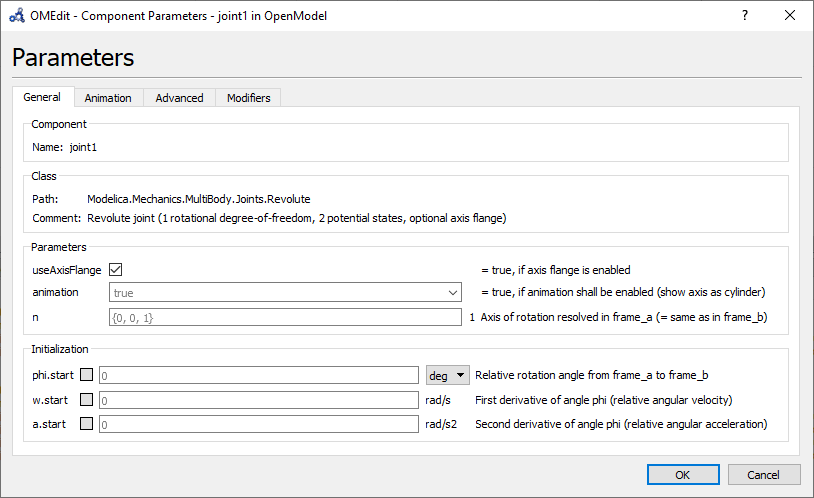
\includegraphics[width=3.5in]{./images/Joint1Parameters}}
\caption{OpenModelica, Joint1 parameters.\label{Joint1Parameters}}
\end{figure}

\begin{figure}
\centerline{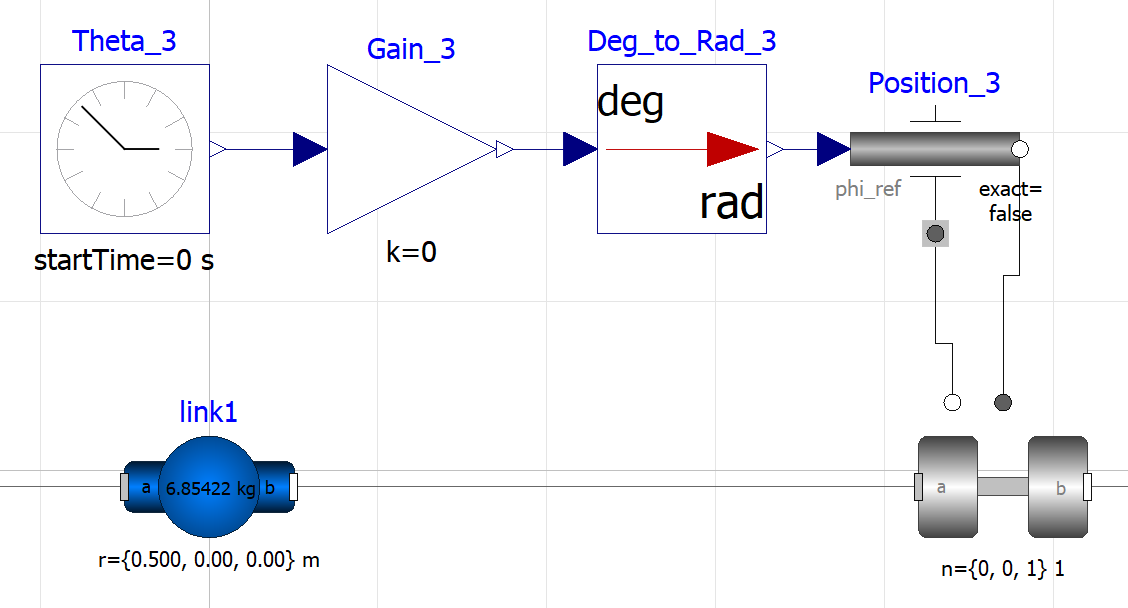
\includegraphics[width=3.5in]{./images/Joint1Link1+Controller}}
\caption{Joint1, Link1 and controller.\label{Joint1Link1+Controller}}
\end{figure}


The CAD modeling software chosen was SolidWorks from Dassault Systems, It is a solid modeling computer-aided design software with 2.3 million active users at over 234,800 companies in 80 countries. \cite{ref5} SolidWorks goal is building 3D CAD software that was easy-to-use, affordable, and available on Windows. \cite{ref6}
The main reasons to use SolidWorks in this project were the easy of use, the calculations that can be used as OpenModelica parameters and the exporting features that allows easy integration between the two software.

An import aspect of exporting from Solidworks to OpenModelica is the compatibility, the exported file can be a $.STL$ file. Although the measurements have to be in meters.
In the $STL$ exporting window there is the option "Do not translate $STL$ output data to positive space", this option makes exported parts maintain their original position in global space, relative to the origin \cite{ref4}. 

There are many ways to export from one software to the other, on this project approach, at the export STL window, the coordinate system is been output, as can be seen in the import parameters for link 1 on Figure \ref{exportSolidworks}, by exporting the coordinate system placed on the frame position, Figure \ref{Link1Model}, the vector from frame $\{A\}$ to the shape origin, resolved in $\{A\}$ is equal to 0, because the frame coordinate system exported is located at the origin.

We can use the center of mass directly from SoildWorks as well as use the exact distance between the frames at the $r$ parameter as shown in the Figure \ref{Link1Parameters} and Figure \ref{importOpenModelicaParameters}.



\begin{figure}
\centerline{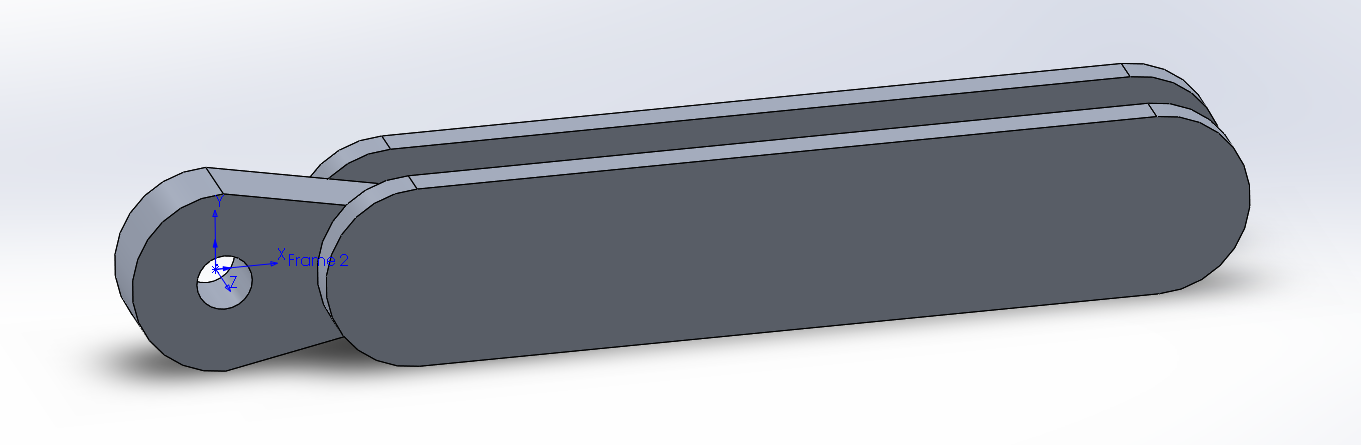
\includegraphics[width=3.5in]{./images/Link1Model}}
\caption{Coordinate system on the frame $\{4\}$ position for link 1.\label{Link1Model}}
\end{figure}

\begin{figure}
\centerline{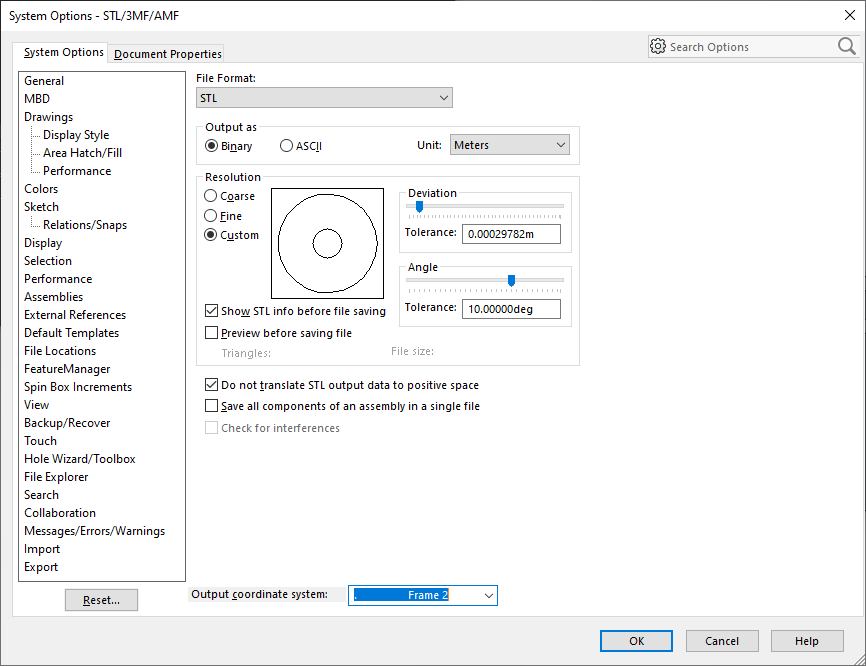
\includegraphics[width=3.5in]{./images/exportSolidworks}}
\caption{Exporting parameters.\label{exportSolidworks}}
\end{figure}

\begin{figure}
\centerline{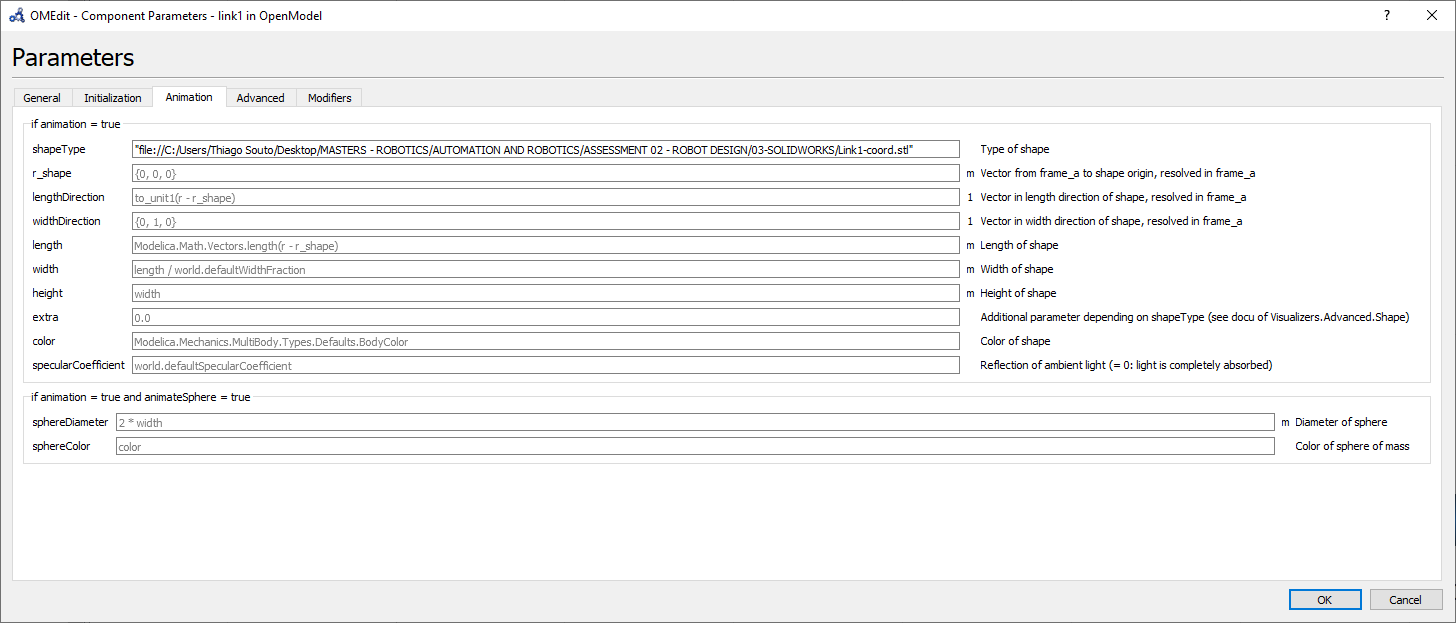
\includegraphics[width=3.5in]{./images/importOpenModelicaParameters}}
\caption{Importing parameters.\label{importOpenModelicaParameters}}
\end{figure}


The calculations for the moments of inertia were made in Python, refer to Appendix \ref{appendix-A}, and confirmed in the mass evaluation at SolidWorks, also, in OpenModelica, as can be seen see on Figure \ref{taus} the values for the torque for joint 1 and 2 using $\theta_{1-4}$ = $0^{\circ}$.

\begin{figure}
\centerline{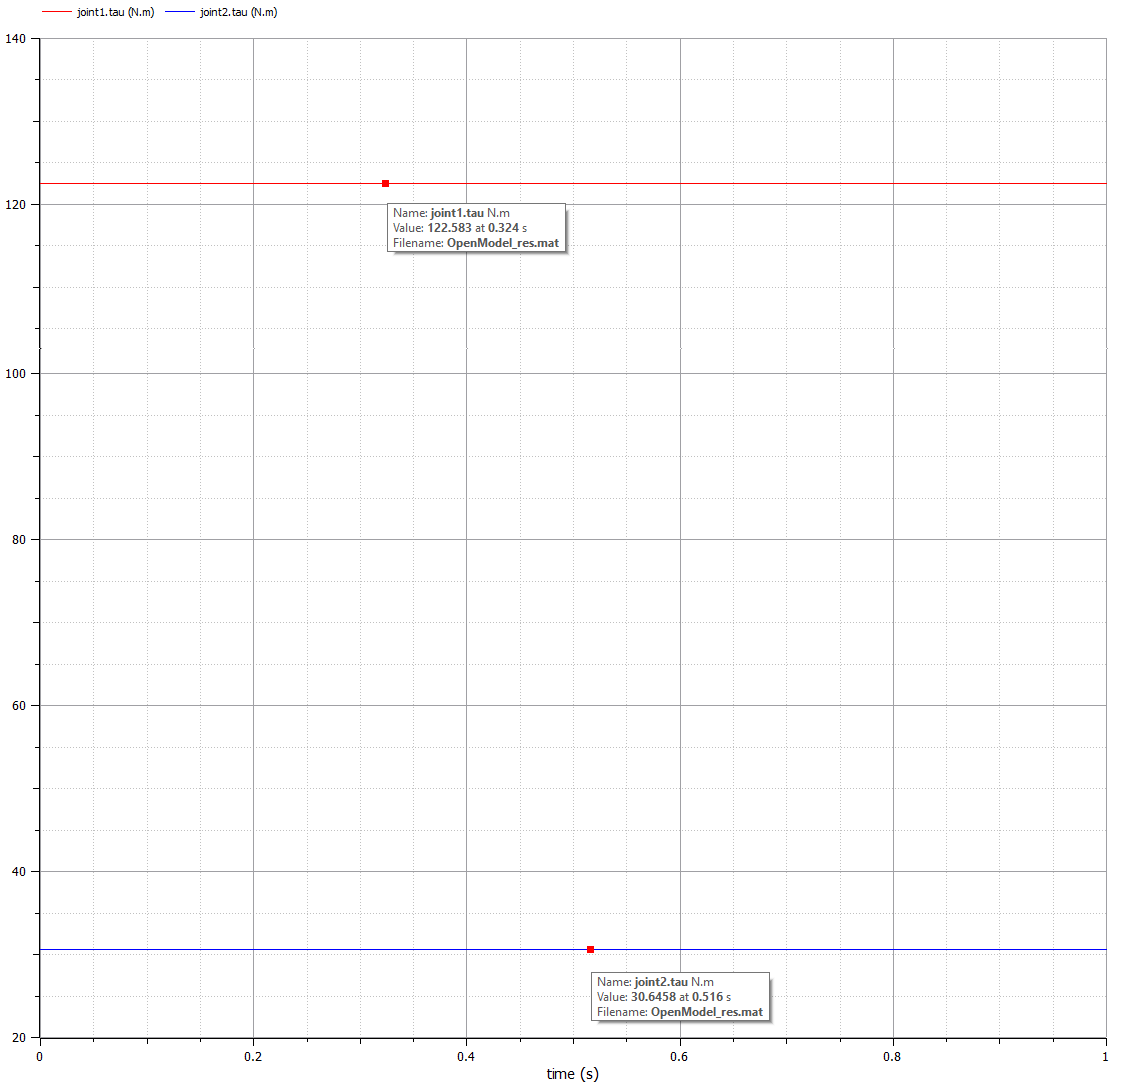
\includegraphics[width=3.5in]{./images/taus}}
\caption{Torques required for $\theta_{1-4}$ = $0^{\circ}$.\label{taus}}
\end{figure}


At Figure \ref{Simulation} the simulation modelling at OpenModelica is shown, the parameters used at the $Gain$ block results in an animation, Figure \ref{SimulationAnimation}, that goes from all the angles been 0 to the values set.

\begin{figure*}
\centerline{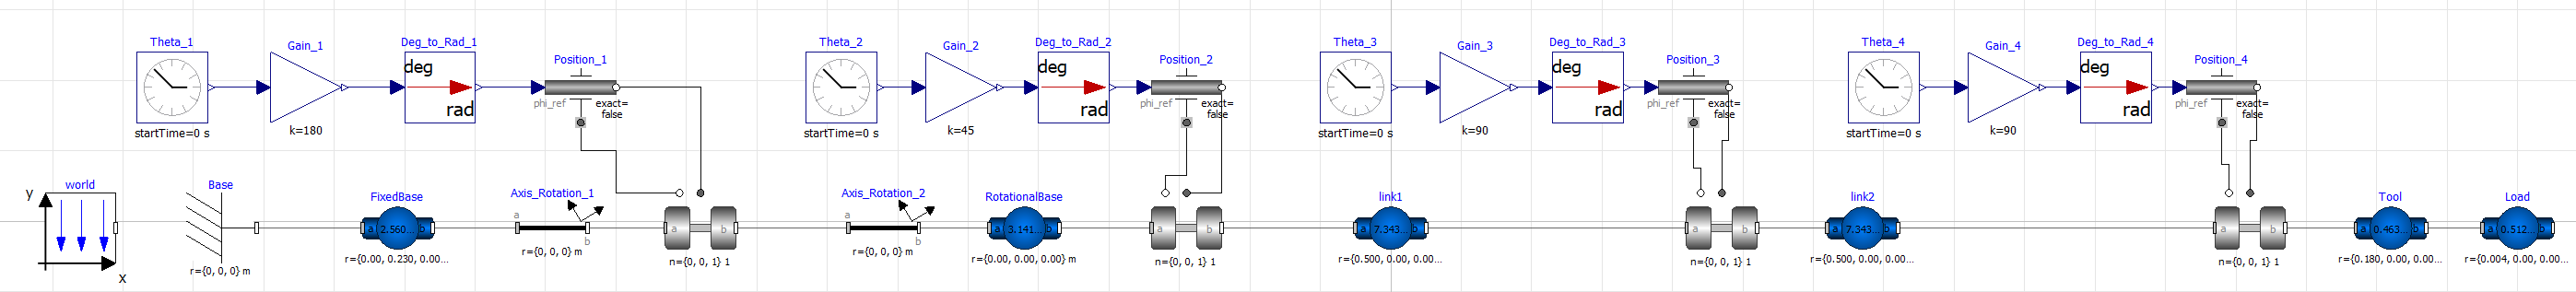
\includegraphics[width=7in]{./images/Simulation}}
\caption{Simulation model, Base, rotational link and 2 more links.\label{Simulation}}
\end{figure*}


\begin{figure*}
\centerline{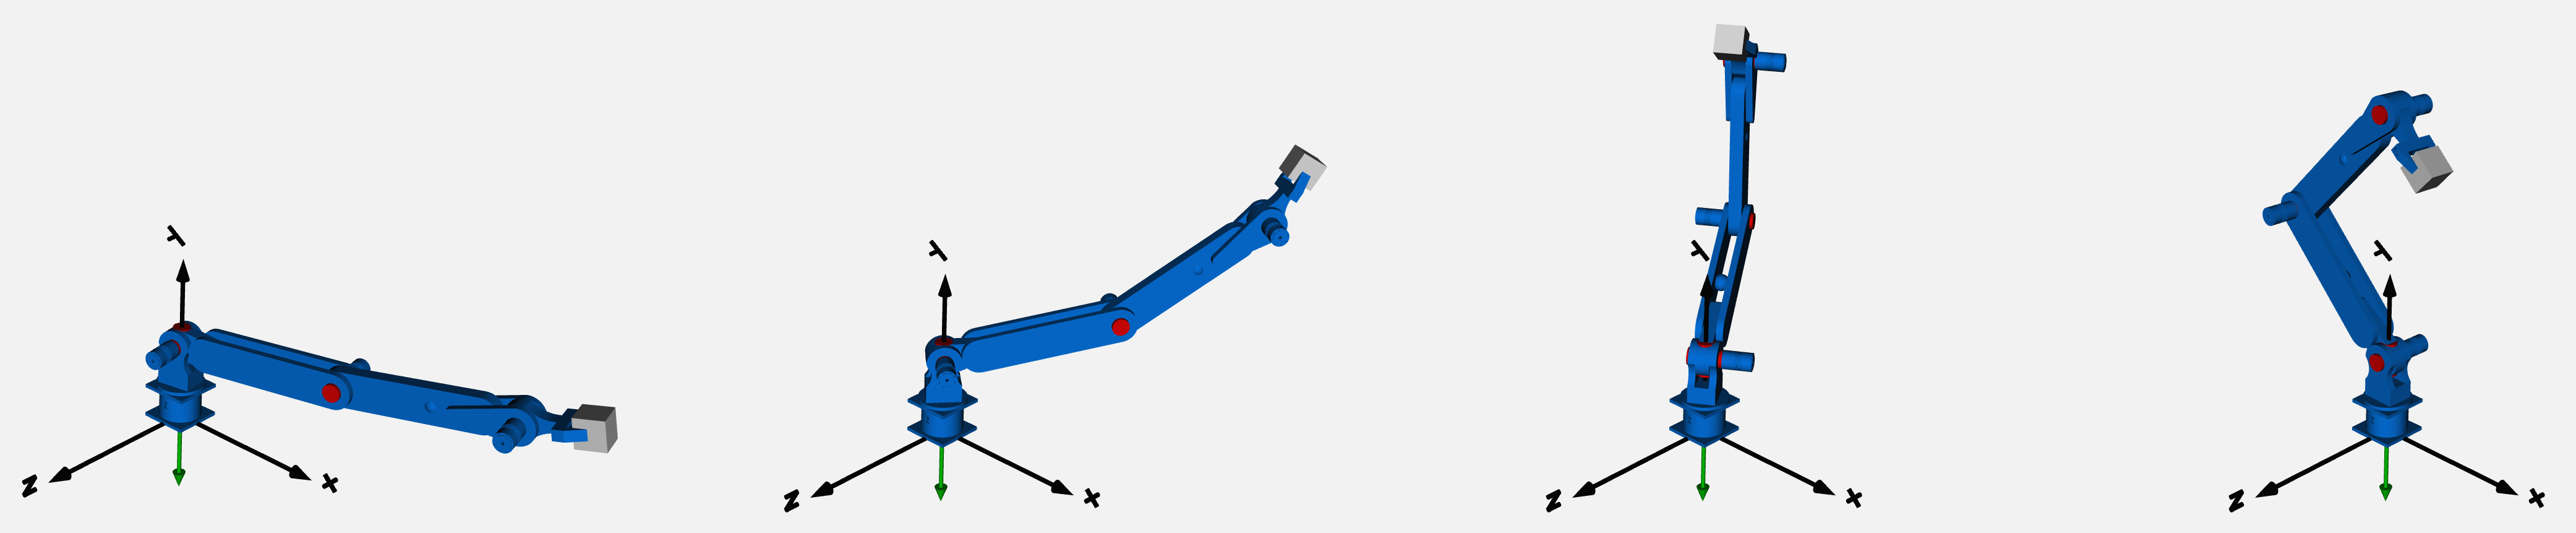
\includegraphics[width=7in]{./images/SimulationAnimation}}
\caption{Simulation animation.\label{SimulationAnimation}}
\end{figure*}









\subsection{Solidworks Simulation}

A Solidworks simulation of the manipulator picking a box on a conveyor and placing it in another conveyor is shown on the electronic report, to see the report follow this \textcolor{blue}{\href{https://thiagosoutogit.github.io/Masters/Pages/Automation/Assessment02RoboticArm.html}{link}}.







\section{Discussion and Conclusions}

Robot manipulators are huge contributor for the robot revolution and will continue to push the industry ahead. The study of it's components and the interactions between them are very important to predict if the designed manipulator will be able to accomplish the task for what it is purposed. New tools for simulation of these robots are improving every day and with such tools, in this project, we were able to demonstrate the design of a robotic manipulator capable of picking objects as well as its forward and inverse kinematics equations. Further developments will include an interface to control the manipulator with real time calculations displayed with the aim of better understand the variables of such an interesting and important tool.


\clearpage
\newpage

\begin{thebibliography}{00}
\bibitem{ref1} J. J. Craig, \emph{Introduction To Robotics: Mechanics And Control}, 3rd ed., Ed. New York: Pearson Education, 2009.

\bibitem{ref2} P. Fritzson, et al. \emph{The OpenModelica Integrated Modeling, Simulation and Optimization Environment} (Conference paper), PROCEEDINGS OF THE 1ST AMERICAN MODELICA CONFERENCE$. $Cambridge, USA: Massechusetts, 2018.

\bibitem{ref3} W. Bolton, \emph{Mechatronics - Electronic control systems in mechanical and electrical engineering}. United Kingdom: Pearson Education Limited, 2019.

\bibitem{ref4} (SOLIDWORKS Online Help) Dassault Systems. (2020, May).  Available: https://help.solidworks.com/.

\bibitem{ref5} (The SOLIDWORKS blog) Dassault Systems. (2020, May).  Available: https://bloHello Rhys,

Thanks gs.solidworks.com/solidworksblog/2016/10/growing-solidworks-nation.html.

\bibitem{ref6} (SolidWoks - Wikipedia)(2020, May). Available: https://en.wikipedia.org/wiki/SolidWorks. 

\bibitem{ref7} K.N. Frazer, School of Food and Advanced Technology, Massey University, Slides from Lecture 12, March 2019.

\bibitem{ref8} \emph{RDrive Datasheet} ROZUM Robotics LLC., Mountain House, CA - USA, 2020.

\bibitem{ref9} (Atan2 - Wikipedia)(2020, May). Available: https://en.wikipedia.org/wiki/Atan2
\end{thebibliography}



\clearpage
\newpage


\appendix
\label{appendix-A}



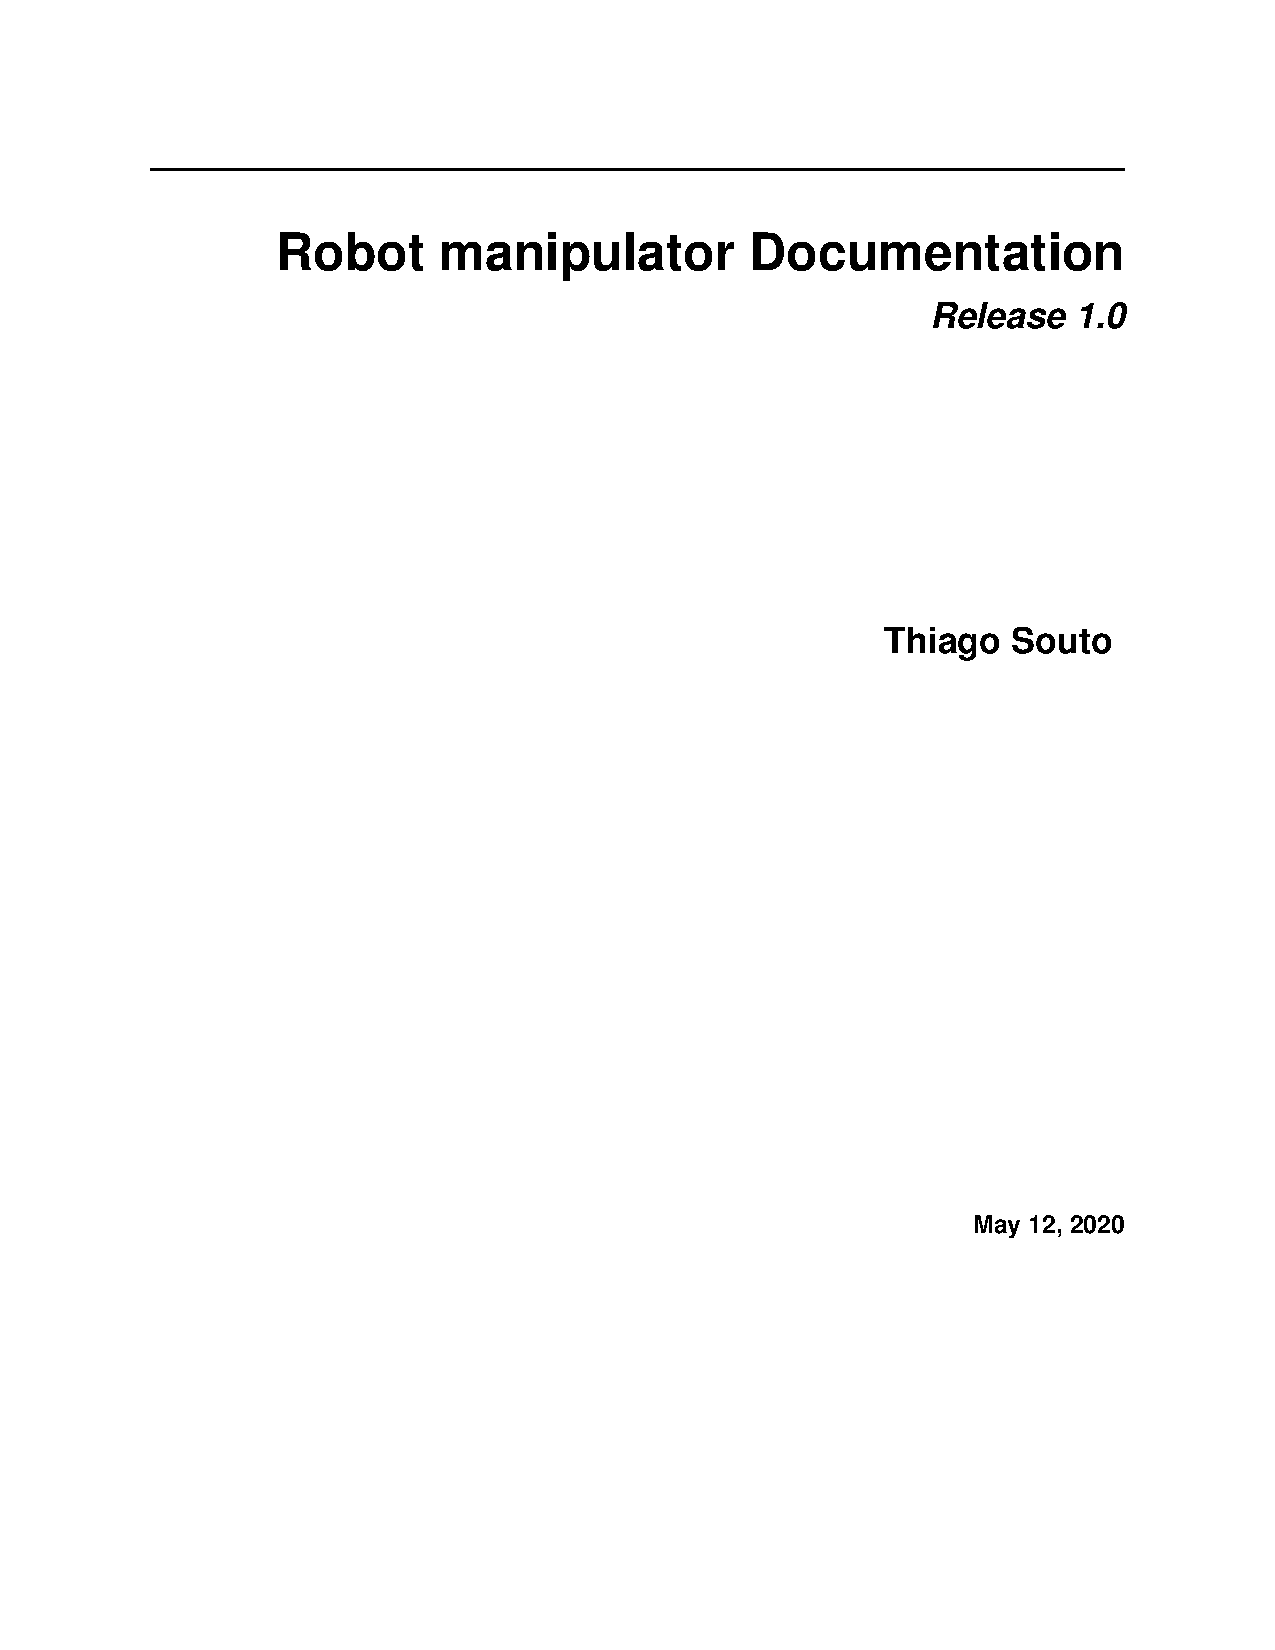
\includepdf[pages=-, frame=false, fitpaper=true, lastpage=8, scale=1, pagecommand={\thispagestyle{plain}}]{./images/MatricesManipulation.pdf}



\end{document}
